%%
%%	AVISO IMPORTANTE
%%	Formato optimizado para el sistema operativo GNU/Linux 64 bits
%%	usar TexLive 2016 (o superior), http://www.ctan.org/tex-archive/systems/texlive/Images/
%%	usar TeXstudio 2.11, http://texstudio.sourceforge.net/
\PassOptionsToPackage{english, spanish}{babel} %Before \documentclass because of clash with babel
\documentclass[letterpaper,12pt]{thesisECFM}
\usepackage{macros}
\usepackage[utf8]{inputenc}
%\usepackage[english, spanish]{babel}
\usepackage[fixlanguage]{babelbib}
\usepackage{url}
\usepackage{hyperref}
\usepackage{comment}
\usepackage{graphicx}
\usepackage{tabularx}
\usepackage{subfig}
\usepackage{amssymb}
\usepackage{mathtools}
\usepackage{amsthm}
\usepackage{todo}
%\usepackage{cleveref}
%\usepackage{xcite}
%\usepackage{xr}
%\externaldocument{Tsunamis}

%% Opciones para los paquetes
\mathtoolsset{showonlyrefs=true} %true for numbering only referenced equations, false otherwise

%%	NO OLVIDE INCLUIR FUENTE DE LAS TABLAS Y FIGURASotas

% Decomentar para anular recuadros en los hiperenlaces dentro del pdf
% \hypersetup{pdfborder={0 0 0}}

% Teoremas ---------------------------------------------------------
% estos ambientes son para teoremas, lemas, corolarios, otros
% si no los utiliza los puede obviar en su trabajo de graduación
%\theoremstyle{plain}
%\newtheorem{thm}{Teorema}[section]
%\theoremstyle{definition}
%\newtheorem{exa}{Ejemplo}[chapter]
%\theoremstyle{remark}
%\newtheorem{rem}{Nota}[chapter]

% Operadores y funciones -------------------------------------------
% Los siguientes son ejemplos de comandos definidos por el usuario
% puede borrarlos, únicamente están para mostrar cómo se construyen con LaTeX
%\DeclareMathOperator{\Supp}{Supp}       \DeclareMathOperator{\vol}{Vol}%
\DeclareMathOperator{\surface}{surface}
\DeclareMathOperator{\bottom}{bottom}
\DeclareMathOperator{\atm}{atm}
%\DeclareMathOperator{z_{\bottom}}{b}
%\newcommand{\Hi}{\mathcal{H}}           \newcommand{\Ba}{\mathcal{B}}%
%\newcommand{\norm}[1]{\left\Vert#1\right\Vert}
%\newcommand{\union}[4]{\bigcup_{{#2}={#3}}^{#4} #1_{#2}}
\newcommand{\intver}{\int_{\zbot}^{\sup}}
\newcommand{\vol}{\Omega} %volume
\newcommand{\bup}{\eta} %bottom uplift
\renewcommand{\sup}{\xi} %surface uplift
\newcommand{\down}{H} %bottom bathymetry
\newcommand{\zbot}{z_b} %Sea bottom = -H + bup
%\newcommand{\zbot}{H} %Sea bottom = -H + bup
%\newcommand{\up}{z_0}

%\newcommand{\ddt}{\frac{d}{dt}}
\newcommand{\ddt}[1]{\frac{d #1}{dt}}
\newcommand{\pddt}[1]{\frac{\partial #1}{\partial t}}
\newcommand{\pddx}[1]{\frac{\partial #1}{\partial x}}
\newcommand{\pddy}[1]{\frac{\partial #1}{\partial y}}
\newcommand{\pddz}[1]{\frac{\partial #1}{\partial z}}
\renewcommand{\div}[1]{\nabla \cdot \left( #1 \right)}
\renewcommand{\v}[1]{\vec{#1}}
\renewcommand{\rvert}[1]{\,\raisebox{-.5em}{$\vert_{#1}$}}
\newcommand{\D}{\Delta}
\newcommand{\then}{\Rightarrow}
%%%%%%%%%%%%%%%%%%%%%%%%%%%%%%%%%%%%%%%%%%%%%%%%%%%%%%%%%%%%%%%%%%%%

\graphicspath{{../Images/}{/home/joshy/Pictures/}}

% Cuerpo de la tesis -----------------------------------------------
\usepackage{subfiles} %doc says this should be included last in the preamble, dunno why
\begin{document}

%% Datos generales del trabajo de graduación
\datosThesis%
{1}%						% física 1; matemática 2
{ En busca de un Mundo Feliz a través de la Geometría Diferencial}%		% Título del trabajo de graduación
{Fulano de Tal}%			% autor
{Mengano Pérez}%			% asesor
{septiembre de 2015}		% mes y año de la orden de impresión
{2}							% femenino 1; masculino 2

%% Datos generales del examen general privado
\examenPrivado%
{M.Sc. Edgar Anibal Cifuentes Anléu}%	% director ECFM
{Ing. José Rodolfo Samayoa Dardón}%		% secretario académico
{Perengano}%		% examinador 1
{Zutano}%		% examinador 2
{Fulano 2}%		% examinador 3

{\onehalfspacing	% interlineado 1 1/2

\OrdenImpresion{ordenImpresion}		% incluye orden de impresión, guardada en pdf

%\Agrade{agradecimientos}			% Agradecimientos

%\Dedica{dedicatoria}				% Dedicatoria

\par}
 
\frontmatter    % --------------------------------------------------  Hojas preliminares

{\onehalfspacing	% interlineado 1 1/2

\tableofcontents    % Índice general vinculado

%%% \figurasYtablas{ lista_figuras }{ lista_tablas }; con valor 1 se incluye la lista,
%%% cualquier otro valor no la genera
%\figurasYtablas{1}{1}

%%%% INCLUYA LA SIMBOLOGÍA NECESARIA EN ESTE APARTADO
%%% NO CAMBIAR LA DEFINICIÓN DE LA TABLA LARGA


\chapter{LISTA DE SÍMBOLOS}

\begin{longtable}{@{}l@{\extracolsep{\fill}} p{4.75in} @{}}  %%%	NO CAMBIAR ESTA LÍNEA
  \textsf{Símbolo} & \textsf{Significado}\\[12pt]
  \endhead
  $:=$ & es definido por\\
  $\cong$ & es isomorfo a\\
  $\Leftrightarrow$ & si y sólo si\\
  $\varnothing$ & conjunto vacío\\
  $E^c$ & complemento de $E$\\
  $\varsubsetneq$ & estrictamente contenido\\
  $E\setminus F$ & diferencia entre $E$ y $F$\\
  $E\Delta F$ & diferencia simétrica entre $E$ y
  $F$\\
  $\mathcal{P} (X)$ & conjunto potencia de $X$\\
  $\chi_E$ & función característica de $E$\\
  $E_n\!\!\uparrow$ & $E_n$ es una sucesión
  creciente\\
  $\mathfrak{L}$ & \salg{} de los conjuntos
  Lebesgue"=medibles\\
  $\mathscr{S}$ & espacio muestral\\
  $\mathfrak{A}$ & \salg{} de eventos\\
  $(\mathscr{S},\mathfrak{A},P)$ & espacio de
  probabilidad\\
  $\mathscr{D}$ & espacio de las funciones de
  prueba\\
  $\mathscr{D}'$ & espacio de las distribuciones\\
  $\delta_0$ & medida de Dirac, función $\delta$ de Dirac o
  $\delta$-función\\
  $\Phi^{\times}$ & espacio antidual de $\Phi$\\
  $\Phi\subset \mathcal{H}\subset \Phi^{\times}$ &
  espacio de Hilbert equipado o tripleta de Gel'fand\\
  $\left\vert \psi \right>$ & vector \emph{ket}\\
  $\left< \psi \right\vert$ & funcional \emph{bra}\\
  $\left< \varphi \vert \psi \right>$ & \emph{braket}
\end{longtable}
  % Lista de símbolos

%%%% Haga el diseño que más le guste
\chapter{OBJETIVOS}

\section*{General}
Escriba el objetivo general.


\section*{Específicos}
Enumere los objetivos específicos.
\begin{enumerate}
\item 
\item 
\end{enumerate}

      % Resumen y objetivos

%%%% Haga el diseño que más le guste
\chapter{INTRODUCCIÓN}


      % Introducción



\mainmatter     % --------------------------------------------------  Cuerpo del Trabajo de Graduación
%\subfileinclude{Tsunamis}
%\subfile{Tsunamis}
%\documentclass[TesisTotal.tex]{subfiles}
%\begin{document}
\chapter{Tsunamis en Guatemala}

\section{Tsunamis}
Un tsunami es, en términos generales, una serie de olas generadas a partir de un movimiento abrupto de gran magnitud en el fondo del mar, el cual se propaga verticalmente hasta la superficie\cite{tsunamiGlossary}. En la mayoría de los casos, este movimiento es ocasionado por un sismo de poca profundidad en una placa oceánica, pero también puede ser causado por otras fuentes, como distintos tipos de sismicidad (incluyendo sismos en placas continentales), actividad volcánica, un deslizamiento en el relieve oceánico o el impacto de un meteorito en el océano\cite{posterGlobal, posterCA, OLoughlin_etal2013}.
La amplitud de estas olas, al llegar a las costas, puede variar de entre algunos centímetros hasta varios metros.
Dependiendo de la magnitud del evento, estas olas pueden traer consigo varios escombros; tales como embarcaciones, grandes volúmenes de arena y objetos arrastrados por el agua en su trayectoria\cite{tsunamiGlossary}.

Estas olas pueden recorrer grandes distancias, pudiendo llegar a recorrer mares completos\cite{tsunamiGlossary}. 
El tiempo de arribo de dichas olas a las costas puede variar entre algunos minutos y unas cu\'antas horas. En Guatemala, aunque el dato no está concensuado, se estima que este tiempo de arribo, en los peores escenarios, puede ser del orden de 15 minutos.
Con este tiempo es factible realizar alertas tempranas para la evacuación de comunidades.

En Guatemala, estas alertas son recibidas del Centro de Alerta de Tsunamis del Pacífico (PTWC, por sus siglas en inglés) y del Centro de Asesoramiento de Tsunami para América Central (CATAC), y posteriormente transmitidas a la población.
La autoevacuación es siempre recomendada\cite{PNR}: al sentir un sismo de gran intensidad, correr hacia puntos seguros previamente identificados. De no ser posible evacuar hacia puntos con suficiente elevación, se recomienda buscar edificaciones altas con cimientos fuertes, o incluso trepar un 
árbol con tronco fuerte\cite{lessonsIndonesia,lessonsCHJ}.


La simulación de tsunamis se hace en tres etapas: generación, propagación e inundación.

\subsection{Propagación: ecuaciones de agua poco profunda}

Consideramos un cuerpo finito de agua con volumen $\vol$, densidad $\rho$ y velocidad $\v{v}$ dada por
\begin{equation}
  \label{eq:v}
  \vec{v} = u \hat{i} + v \hat{j} + w \hat{k} = (u,v,w).
\end{equation}

El cuerpo se encuentra aislado, de manera que su masa ($m$) se conserva, siguiendo la ecuación:

\begin{equation}
  \frac{ \partial \rho}{\partial t} + \nabla \cdot (\rho \vec{v}) = 0
  \label{eq:continuidad}
\end{equation}

\begin{proof} \todo{A esto le falta mucho para ser una demostración formal. Quisiera hacer una, pero me puede tomar mucho tiempo, aunque considero que vale la pena. Me hace sentr más seguro de lo que digo, me ayuda a simplificar la redacción y me permite hacer cambios sin afectar la continuidad del tema.}
Consideremos un flujo de masa en un volumen infinitesimal $dV$ dentro de $\vol$, dado por $\frac{dm}{dt} = \frac{\partial m}{\partial V} \frac{dV}{dt}$.
Para un volumen infinitesimal, podemos considerar que el fluído se mueve en una sola dirección $\hat{n}$, de manera que el volumen de fluido desplazado en el tiempo $dt$ es $A d\vec{s} \cdot \hat{n}$, y $\frac{dm}{dt} = \int_{\vol} \frac{\partial m}{\partial V} \frac{d\vec{s}}{dt} \cdot \hat{n} {dA} = \int_{\vol} \rho \vec{v} \cdot \hat{n} dA $, donde $\rho$ representa la densidad del fluído, $A$ el área transversal de $dV$, y $\vec{v}$ la velocidad del fluído en $dV$.\\
Esta ecuación es similar a la del flujo total de una cantidad $q$ dada por una densidad de flujo $\vec{j}$: $\frac{dq}{dt} = \int_{d\vol} \vec{j} \cdot \hat{n} dA$. En este caso, $q = m$ y $\vec{j} = \rho \vec{v}$. \todo{En realidad hay un signo mal en algún lugar de aquí, ¿$\vec{j}$ va hacia adentro o hacia afuera de $dV$? Creo que en la ecuación de flujo va hacia adentro, y en la de continuidad va hacia afuera.}\\
Expresando $\frac{dm}{dt}$ como $\frac{d}{dt} \int_\vol \rho dV$ y convirtiendo la integral $\int_{d\vol} \vec{j} \cdot \hat{n} dA$ a una integral volumétrica por medio del teorema de Gauss, llegamos a la conocida ecuación de continuidad: \footnote{Aquí hay un paso oculto, puesto que $\frac{d\vol}{dt} \neq 0$, en cuyo caso (ver teorema de Reynolds):  $\frac{d}{dt} \int_\vol \rho dV =\int_\vol \left( \frac{\partial \rho}{\partial t} + \nabla \cdot (\rho \vec{v}) \right) dV$, así que hay que demostrar que $\nabla \cdot (\rho \vec{v}) = 0$ para llegar a la ecuación citada. Esto se demuestra más adelante. \todo{En realidad no tiene sentido tener que demostrar eso antes, porque ese es precisamente el resultado que se quiere obtener de esa ecuación. Podría escribir la ecuación como $\frac{ \partial \rho}{\partial t} + 2 \nabla \cdot (\rho \vec{v}) = 0$, pero no encuentro eso en ninguna referencia, así que me da miedo ponerlo. En todo caso, si la escribiera así, tendría que cambiar la expresión ``...la conocida ecuación...''.}}
\[
  \frac{ \partial \rho}{\partial t} + \nabla \cdot (\rho \vec{v}) = 0
\]
\end{proof}

El cuerpo está sujeto a una fuerza gravitacional $\int_{\vol} \rho \vec{g} dV$, y su propia presión como fuerza de contacto: $\int_{d\vol} -\vec{p} \cdot \hat{n} dA$; de manera que, siguiendo la ley de conservación de momentum lineal, obtenemos las ecuaciones clásicas de Navier-Stokes: \todo{¿Quitar el paréntesis? Tendría que cambiar $\div{v}$ por la expresión completa}

\begin{equation}
  \label{eq:Navier-Stokes}
  \pddt{} (\rho \v{v}) +(\v{v}\cdot\nabla)(\rho\v{v}) = -\nabla p + \rho \v{g} + \rho \v{v} (\div{\v{v}}) - 2 \v{\Omega} \times \v{v}
\end{equation}

Para el caso del mar, puede considerarse que sigue un flujo incompresible; es decir, para un volumen infinitésimal que se mueve con el fluído, se cumple que $\pddt{\rho} = \nabla \rho =  0$.\todo{buscar referencia}
% Durante la propagación en mar profundo, consideraremos únicamente desplazamientos verticales pequeños \todo{Este no es el argumento real. No recuerdo cuál es y ya tengo mucho sueño :(}, por lo que podemos
%En el caso de un fluído incompresible ($\frac{\partial \rho}{\partial p}=0$), podemos asumir $\pddt{\rho} = \nabla \rho =  0$, de modo que, según la ecuación \eqref{eq:continuidad},

Considerando esto en la ecuación de continuidad \eqref{eq:continuidad}, legamos a:

\begin{equation}
  \label{eq:divV}
  \div{v}=0  
\end{equation}


Así, según \eqref{eq:Navier-Stokes}:
\begin{equation}
  \label{eq:Navier-Stokes2}
  \pddt{\v{v}} + (\v{v}\cdot\nabla)\v{v} = \frac{-\nabla p}{\rho} + \v{g} - \frac{2 \v{\Omega} \times \v{v}}{\rho}
\end{equation}

\subsubsection{Condiciones de frontera}
\label{sec:condiciones-frontera}

Consideremos ahora el caso de un desplazamiento vertical en el fondo del mar dado por $\bup$ con respecto a su profundidad en estado estable $\down$, el cual genera un desplazamiento vertical en la superficie dado por $\sup$. Ver figura \ref{fig:upLift}.

\begin{figure}
  \centering
  \includegraphics[width=.8\linewidth]{upLift}
  \caption{Desplazamiento vertical $\bup$ en el fondo del mar, generando un desplazamiento $\sup$ de la superficie con respecto a su altura en estado estable $\down$. Fuente: \cite{Levin2016}}
  \label{fig:upLift}
\end{figure}

La superficie del mar será siempre una función continua de $(x,y,t)$: $z_{\surface} = \sup(x,y,t)$
, de manera que el flujo superficial cumple la condición
\begin{equation}
  \label{eq:freeSurfaceFlow}
  \ddt{}z_{\surface} = w \rvert{z=\sup} = \pddt{\sup} + u \pddx{\sup} + v \pddy{\sup}.
\end{equation}

Además, por continuidad, la presión en la superfice debe ser igual a la presión atmosférica:

\begin{equation}
  \label{eq:p_atm-continuity}
  p \rvert{z=\sup} = p_{\atm}
\end{equation}

Mientras, en el fondo del mar, el único cambio en $z$ estará dado por $\bup$: $z_{\bottom} = \zbot = -\down(x,y) + \bup(x,y,t)$, de manera que el flujo normal cumple la condición
\begin{equation}
  \label{eq:normalFlow}
    \ddt{}\zbot = w \rvert{z=\zbot} = -u \pddx{\down} - v \pddy{\down} + \ddt{\bup}
\end{equation}

Para un proceso instantáneo, podemos considerar únicamente deformaciones residuales. En este caso:

\begin{equation}
  \label{eq:w-bottom-instantaneous}
  w \rvert{z=\zbot} = -u \pddx{\down} - v \pddy{\down}
\end{equation}


Y, dado que en $\zbot$ no puede haber movimiento vertical además de $\bup$, se debe cumplir la condicón:

\begin{equation}
  \label{eq:no-normal-flow}
  \v{v} \cdot \hat{n} = \v{v}_\bup \cdot \hat{n}
\end{equation}

Donde $\v{v}_\bup = \ddt{\zbot}$. %representa la velocidad con que se levanta el fondo del mar luego del movimiento del suelo.

\subsubsection{Ecuación de continuidad promedio}
\label{sec:depth-average-continuity-equation}

Integrando la ecuación \eqref{eq:divV} verticalmente:
\begin{eqnarray}
  \label{eq:2}
  \intver \div{v} \, dz & = & \intver \left( \pddx{u} + \pddy{v} \right) dz + w\rvert{z=\sup} - w \rvert{z=\zbot} \\
                        & = & \pddx{} \intver u \, dz + \pddy{} \intver v \, dz - 
                              \left(
                              u\rvert{z=\sup} \pddx{\sup} + u \rvert{z=\zbot} \pddx{\zbot}
                              \right)\\ & &
  -                              \left( 
  - v \rvert{z=\sup} \pddy{\sup} + v \rvert{z=\zbot} \pddy{\zbot}
  \right)
                                            + w \rvert{z=\sup} - w_{\bottom}
%                              \right)
\end{eqnarray}

Identificamos los primeros términos entre paréntesis de la ecuaci\'on anterior como $w \rvert{z=\zbot}$, y los segundos como $w\rvert{z=\sup} + \pddt{\zbot}$; de modo que, definiendo $\hat{u} = \frac{1}{\zbot} \intver u \, dz$ y $\hat{v} = \frac{1}{\zbot} \intver v \, dz$, llegamos a la ecuación de continuidad promedio:

\begin{equation}
  \label{eq:depth-average}
  \pddt{\zbot} + \pddx{\zbot \bar{u}} + \pddy{\zbot \bar{v}} = 0
\end{equation}

\subsubsection{Long wave approximation}
\label{sec:longwaveapprox}

Expandiendo la ecuación \eqref{eq:divV}:
\begin{equation}
  \label{eq:divergence}
  \pddx{u} + \pddy{v} + \pddy{z} = 0  
\end{equation}

Si asumimos $u \sim v$, en media longitud de onda $0.5 \lambda $, correspondiente a un desplazamiento vertical $\down$, notamos que

\begin{equation}
  % \label{eq:longWaveAprox}
\label{eq:1}
  \frac{\D u}{0.5 \lambda} + \frac{\D u}{0.5 \lambda} + \frac{\D w}{\down} = 0 \then |\D w| \sim \frac{\down}{\lambda} | \D u |
\end{equation}

De modo que, si $H << \lambda$, $\D w$ puede ser descartado al estar acompañado por trémino del orden de $\D u$.
Esta aproximaci\'on es conocida como aproximación de ondas largas (\textit{long wave approximation}).

Además, consideremos la fuerza de Coriolis en la ecuación \eqref{eq:Navier-Stokes2};
en el caso de la rotación de la Tierra, $\Omega = (0, \omega co(\phi), \omega sin(\phi)$, donde $\omega$ represena la rapidez de rotación y $\phi$ la latitud del punto en consideraci\'on,
%Usando \eqref{eq:v}, llegamos a:

\begin{eqnarray}
  \label{eq:coriolis-approx-0}
  2 \v{\Omega} \times \v{v} = & 2 \omega (v \sin \phi - w \cos \phi, -u \sin \phi, u \cos \phi) \\
  \approx & 2 \omega ( v \sin \phi, -u \sin \phi, 0 ) % \\  = & 2 \omega (fv,-fu)
\end{eqnarray}

%Donde definimos $f = 2 \omega \sin \phi$,
El término $ \omega w \cos \phi$ es despreciado en comparación con $ \omega v \sin \phi$, y el término de aceleración vertical ($ \omega u \cos \phi$) es despreciado en comparación con $\v{g}$.
Definiendo $f = 2 \omega \sin \phi$, reescribimos la fuerza de Coriolis como:

\begin{equation}
  \label{eq:CoriolisApprox}
  2 \v{\Omega} \times \v{v} \approx 2 \omega (fv, -fu)
\end{equation}

Veamos ahora la componente vertical de \eqref{eq:Navier-Stokes2}.
El término $(\v{v} \cdot \nabla) \v{v}$ puede ser descartado en comparaci\'on con \v{g}, al igual que el térmno de la ecuación de Coriolis. Así, para la componente vertical del movimiento del agua, se cumple la ecuación

\begin{equation}
  \label{eq:N-S_z_pre}
  \pddz{p} = -\rho g
\end{equation}

De modo que, integrando de $z$ a $\sup$, considerando la ecuación \eqref{eq:p_atm-continuity}, la presión está dada por

\begin{equation}
  \label{eq:pressure}
  p(x,y,z,t) = p_{atm}+ \rho g (\sup - z)
\end{equation}

Y $\pddx{p} = \pddx{p_{atm}} + \rho g \pddx{\sup}$, y similarmente para $y$.

Con esto, las componentes horizontales de la ecuación \eqref{eq:Navier-Stokes2} se convierten en:

\begin{eqnarray}
  \label{eq:N-S_x}
  \pddt{u} + u \pddx{u} + v \pddy{u} & = & -g \pddx{\sup} -\frac{1}{\rho} \pddx{p} + fv \\
  \pddt{v} + u \pddx{v} + v \pddy{v} & = & -g \pddx{\sup} -g \pddx{p} - fu
\end{eqnarray}

Que son las ecuaciones de aguas poco profundas (\textit{shallow water equations}) con la fuerza de Coriolis y sin considerar viscosidad en el fluído.

%
%\end{document}
%%% Local Variables:
%%% TeX-master: "TesisTotal"
%%% End:
 %both \input and \include seem to work. \input is like a copy-paste; \include handles the included file as a separate file (creating an .aux for the file), which is something I want
%%\documentclass[TesisTotal.tex]{subfiles}
%\begin{document}
\chapter{Tsunamis en Guatemala}

\section{Tsunamis}
Un tsunami es, en términos generales, una serie de olas generadas a partir de un movimiento abrupto de gran magnitud en el fondo del mar, el cual se propaga verticalmente hasta la superficie\cite{tsunamiGlossary}. En la mayoría de los casos, este movimiento es ocasionado por un sismo de poca profundidad en una placa oceánica, pero también puede ser causado por otras fuentes, como distintos tipos de sismicidad (incluyendo sismos en placas continentales), actividad volcánica, un deslizamiento en el relieve oceánico o el impacto de un meteorito en el océano\cite{posterGlobal, posterCA, OLoughlin_etal2013}.
La amplitud de estas olas, al llegar a las costas, puede variar de entre algunos centímetros hasta varios metros.
Dependiendo de la magnitud del evento, estas olas pueden traer consigo varios escombros; tales como embarcaciones, grandes volúmenes de arena y objetos arrastrados por el agua en su trayectoria\cite{tsunamiGlossary}.

Estas olas pueden recorrer grandes distancias, pudiendo llegar a recorrer mares completos\cite{tsunamiGlossary}. 
El tiempo de arribo de dichas olas a las costas puede variar entre algunos minutos y unas cu\'antas horas. En Guatemala, aunque el dato no está concensuado, se estima que este tiempo de arribo, en los peores escenarios, puede ser del orden de 15 minutos.
Con este tiempo es factible realizar alertas tempranas para la evacuación de comunidades.

En Guatemala, estas alertas son recibidas del Centro de Alerta de Tsunamis del Pacífico (PTWC, por sus siglas en inglés) y del Centro de Asesoramiento de Tsunami para América Central (CATAC), y posteriormente transmitidas a la población.
La autoevacuación es siempre recomendada\cite{PNR}: al sentir un sismo de gran intensidad, correr hacia puntos seguros previamente identificados. De no ser posible evacuar hacia puntos con suficiente elevación, se recomienda buscar edificaciones altas con cimientos fuertes, o incluso trepar un 
árbol con tronco fuerte\cite{lessonsIndonesia,lessonsCHJ}.


La simulación de tsunamis se hace en tres etapas: generación, propagación e inundación.

\subsection{Propagación: ecuaciones de agua poco profunda}

Consideramos un cuerpo finito de agua con volumen $\vol$, densidad $\rho$ y velocidad $\v{v}$ dada por
\begin{equation}
  \label{eq:v}
  \vec{v} = u \hat{i} + v \hat{j} + w \hat{k} = (u,v,w).
\end{equation}

El cuerpo se encuentra aislado, de manera que su masa ($m$) se conserva, siguiendo la ecuación:

\begin{equation}
  \frac{ \partial \rho}{\partial t} + \nabla \cdot (\rho \vec{v}) = 0
  \label{eq:continuidad}
\end{equation}

\begin{proof} \todo{A esto le falta mucho para ser una demostración formal. Quisiera hacer una, pero me puede tomar mucho tiempo, aunque considero que vale la pena. Me hace sentr más seguro de lo que digo, me ayuda a simplificar la redacción y me permite hacer cambios sin afectar la continuidad del tema.}
Consideremos un flujo de masa en un volumen infinitesimal $dV$ dentro de $\vol$, dado por $\frac{dm}{dt} = \frac{\partial m}{\partial V} \frac{dV}{dt}$.
Para un volumen infinitesimal, podemos considerar que el fluído se mueve en una sola dirección $\hat{n}$, de manera que el volumen de fluido desplazado en el tiempo $dt$ es $A d\vec{s} \cdot \hat{n}$, y $\frac{dm}{dt} = \int_{\vol} \frac{\partial m}{\partial V} \frac{d\vec{s}}{dt} \cdot \hat{n} {dA} = \int_{\vol} \rho \vec{v} \cdot \hat{n} dA $, donde $\rho$ representa la densidad del fluído, $A$ el área transversal de $dV$, y $\vec{v}$ la velocidad del fluído en $dV$.\\
Esta ecuación es similar a la del flujo total de una cantidad $q$ dada por una densidad de flujo $\vec{j}$: $\frac{dq}{dt} = \int_{d\vol} \vec{j} \cdot \hat{n} dA$. En este caso, $q = m$ y $\vec{j} = \rho \vec{v}$. \todo{En realidad hay un signo mal en algún lugar de aquí, ¿$\vec{j}$ va hacia adentro o hacia afuera de $dV$? Creo que en la ecuación de flujo va hacia adentro, y en la de continuidad va hacia afuera.}\\
Expresando $\frac{dm}{dt}$ como $\frac{d}{dt} \int_\vol \rho dV$ y convirtiendo la integral $\int_{d\vol} \vec{j} \cdot \hat{n} dA$ a una integral volumétrica por medio del teorema de Gauss, llegamos a la conocida ecuación de continuidad: \footnote{Aquí hay un paso oculto, puesto que $\frac{d\vol}{dt} \neq 0$, en cuyo caso (ver teorema de Reynolds):  $\frac{d}{dt} \int_\vol \rho dV =\int_\vol \left( \frac{\partial \rho}{\partial t} + \nabla \cdot (\rho \vec{v}) \right) dV$, así que hay que demostrar que $\nabla \cdot (\rho \vec{v}) = 0$ para llegar a la ecuación citada. Esto se demuestra más adelante. \todo{En realidad no tiene sentido tener que demostrar eso antes, porque ese es precisamente el resultado que se quiere obtener de esa ecuación. Podría escribir la ecuación como $\frac{ \partial \rho}{\partial t} + 2 \nabla \cdot (\rho \vec{v}) = 0$, pero no encuentro eso en ninguna referencia, así que me da miedo ponerlo. En todo caso, si la escribiera así, tendría que cambiar la expresión ``...la conocida ecuación...''.}}
\[
  \frac{ \partial \rho}{\partial t} + \nabla \cdot (\rho \vec{v}) = 0
\]
\end{proof}

El cuerpo está sujeto a una fuerza gravitacional $\int_{\vol} \rho \vec{g} dV$, y su propia presión como fuerza de contacto: $\int_{d\vol} -\vec{p} \cdot \hat{n} dA$; de manera que, siguiendo la ley de conservación de momentum lineal, obtenemos las ecuaciones clásicas de Navier-Stokes: \todo{¿Quitar el paréntesis? Tendría que cambiar $\div{v}$ por la expresión completa}

\begin{equation}
  \label{eq:Navier-Stokes}
  \pddt{} (\rho \v{v}) +(\v{v}\cdot\nabla)(\rho\v{v}) = -\nabla p + \rho \v{g} + \rho \v{v} (\div{\v{v}}) - 2 \v{\Omega} \times \v{v}
\end{equation}

Para el caso del mar, puede considerarse que sigue un flujo incompresible; es decir, para un volumen infinitésimal que se mueve con el fluído, se cumple que $\pddt{\rho} = \nabla \rho =  0$.\todo{buscar referencia}
% Durante la propagación en mar profundo, consideraremos únicamente desplazamientos verticales pequeños \todo{Este no es el argumento real. No recuerdo cuál es y ya tengo mucho sueño :(}, por lo que podemos
%En el caso de un fluído incompresible ($\frac{\partial \rho}{\partial p}=0$), podemos asumir $\pddt{\rho} = \nabla \rho =  0$, de modo que, según la ecuación \eqref{eq:continuidad},

Considerando esto en la ecuación de continuidad \eqref{eq:continuidad}, legamos a:

\begin{equation}
  \label{eq:divV}
  \div{v}=0  
\end{equation}


Así, según \eqref{eq:Navier-Stokes}:
\begin{equation}
  \label{eq:Navier-Stokes2}
  \pddt{\v{v}} + (\v{v}\cdot\nabla)\v{v} = \frac{-\nabla p}{\rho} + \v{g} - \frac{2 \v{\Omega} \times \v{v}}{\rho}
\end{equation}

\subsubsection{Condiciones de frontera}
\label{sec:condiciones-frontera}

Consideremos ahora el caso de un desplazamiento vertical en el fondo del mar dado por $\bup$ con respecto a su profundidad en estado estable $\down$, el cual genera un desplazamiento vertical en la superficie dado por $\sup$. Ver figura \ref{fig:upLift}.

\begin{figure}
  \centering
  \includegraphics[width=.8\linewidth]{upLift}
  \caption{Desplazamiento vertical $\bup$ en el fondo del mar, generando un desplazamiento $\sup$ de la superficie con respecto a su altura en estado estable $\down$. Fuente: \cite{Levin2016}}
  \label{fig:upLift}
\end{figure}

La superficie del mar será siempre una función continua de $(x,y,t)$: $z_{\surface} = \sup(x,y,t)$
, de manera que el flujo superficial cumple la condición
\begin{equation}
  \label{eq:freeSurfaceFlow}
  \ddt{}z_{\surface} = w \rvert{z=\sup} = \pddt{\sup} + u \pddx{\sup} + v \pddy{\sup}.
\end{equation}

Además, por continuidad, la presión en la superfice debe ser igual a la presión atmosférica:

\begin{equation}
  \label{eq:p_atm-continuity}
  p \rvert{z=\sup} = p_{\atm}
\end{equation}

Mientras, en el fondo del mar, el único cambio en $z$ estará dado por $\bup$: $z_{\bottom} = \zbot = -\down(x,y) + \bup(x,y,t)$, de manera que el flujo normal cumple la condición
\begin{equation}
  \label{eq:normalFlow}
    \ddt{}\zbot = w \rvert{z=\zbot} = -u \pddx{\down} - v \pddy{\down} + \ddt{\bup}
\end{equation}

Para un proceso instantáneo, podemos considerar únicamente deformaciones residuales. En este caso:

\begin{equation}
  \label{eq:w-bottom-instantaneous}
  w \rvert{z=\zbot} = -u \pddx{\down} - v \pddy{\down}
\end{equation}


Y, dado que en $\zbot$ no puede haber movimiento vertical además de $\bup$, se debe cumplir la condicón:

\begin{equation}
  \label{eq:no-normal-flow}
  \v{v} \cdot \hat{n} = \v{v}_\bup \cdot \hat{n}
\end{equation}

Donde $\v{v}_\bup = \ddt{\zbot}$. %representa la velocidad con que se levanta el fondo del mar luego del movimiento del suelo.

\subsubsection{Ecuación de continuidad promedio}
\label{sec:depth-average-continuity-equation}

Integrando la ecuación \eqref{eq:divV} verticalmente:
\begin{eqnarray}
  \label{eq:2}
  \intver \div{v} \, dz & = & \intver \left( \pddx{u} + \pddy{v} \right) dz + w\rvert{z=\sup} - w \rvert{z=\zbot} \\
                        & = & \pddx{} \intver u \, dz + \pddy{} \intver v \, dz - 
                              \left(
                              u\rvert{z=\sup} \pddx{\sup} + u \rvert{z=\zbot} \pddx{\zbot}
                              \right)\\ & &
  -                              \left( 
  - v \rvert{z=\sup} \pddy{\sup} + v \rvert{z=\zbot} \pddy{\zbot}
  \right)
                                            + w \rvert{z=\sup} - w_{\bottom}
%                              \right)
\end{eqnarray}

Identificamos los primeros términos entre paréntesis de la ecuaci\'on anterior como $w \rvert{z=\zbot}$, y los segundos como $w\rvert{z=\sup} + \pddt{\zbot}$; de modo que, definiendo $\hat{u} = \frac{1}{\zbot} \intver u \, dz$ y $\hat{v} = \frac{1}{\zbot} \intver v \, dz$, llegamos a la ecuación de continuidad promedio:

\begin{equation}
  \label{eq:depth-average}
  \pddt{\zbot} + \pddx{\zbot \bar{u}} + \pddy{\zbot \bar{v}} = 0
\end{equation}

\subsubsection{Long wave approximation}
\label{sec:longwaveapprox}

Expandiendo la ecuación \eqref{eq:divV}:
\begin{equation}
  \label{eq:divergence}
  \pddx{u} + \pddy{v} + \pddy{z} = 0  
\end{equation}

Si asumimos $u \sim v$, en media longitud de onda $0.5 \lambda $, correspondiente a un desplazamiento vertical $\down$, notamos que

\begin{equation}
  % \label{eq:longWaveAprox}
\label{eq:1}
  \frac{\D u}{0.5 \lambda} + \frac{\D u}{0.5 \lambda} + \frac{\D w}{\down} = 0 \then |\D w| \sim \frac{\down}{\lambda} | \D u |
\end{equation}

De modo que, si $H << \lambda$, $\D w$ puede ser descartado al estar acompañado por trémino del orden de $\D u$.
Esta aproximaci\'on es conocida como aproximación de ondas largas (\textit{long wave approximation}).

Además, consideremos la fuerza de Coriolis en la ecuación \eqref{eq:Navier-Stokes2};
en el caso de la rotación de la Tierra, $\Omega = (0, \omega co(\phi), \omega sin(\phi)$, donde $\omega$ represena la rapidez de rotación y $\phi$ la latitud del punto en consideraci\'on,
%Usando \eqref{eq:v}, llegamos a:

\begin{eqnarray}
  \label{eq:coriolis-approx-0}
  2 \v{\Omega} \times \v{v} = & 2 \omega (v \sin \phi - w \cos \phi, -u \sin \phi, u \cos \phi) \\
  \approx & 2 \omega ( v \sin \phi, -u \sin \phi, 0 ) % \\  = & 2 \omega (fv,-fu)
\end{eqnarray}

%Donde definimos $f = 2 \omega \sin \phi$,
El término $ \omega w \cos \phi$ es despreciado en comparación con $ \omega v \sin \phi$, y el término de aceleración vertical ($ \omega u \cos \phi$) es despreciado en comparación con $\v{g}$.
Definiendo $f = 2 \omega \sin \phi$, reescribimos la fuerza de Coriolis como:

\begin{equation}
  \label{eq:CoriolisApprox}
  2 \v{\Omega} \times \v{v} \approx 2 \omega (fv, -fu)
\end{equation}

Veamos ahora la componente vertical de \eqref{eq:Navier-Stokes2}.
El término $(\v{v} \cdot \nabla) \v{v}$ puede ser descartado en comparaci\'on con \v{g}, al igual que el térmno de la ecuación de Coriolis. Así, para la componente vertical del movimiento del agua, se cumple la ecuación

\begin{equation}
  \label{eq:N-S_z_pre}
  \pddz{p} = -\rho g
\end{equation}

De modo que, integrando de $z$ a $\sup$, considerando la ecuación \eqref{eq:p_atm-continuity}, la presión está dada por

\begin{equation}
  \label{eq:pressure}
  p(x,y,z,t) = p_{atm}+ \rho g (\sup - z)
\end{equation}

Y $\pddx{p} = \pddx{p_{atm}} + \rho g \pddx{\sup}$, y similarmente para $y$.

Con esto, las componentes horizontales de la ecuación \eqref{eq:Navier-Stokes2} se convierten en:

\begin{eqnarray}
  \label{eq:N-S_x}
  \pddt{u} + u \pddx{u} + v \pddy{u} & = & -g \pddx{\sup} -\frac{1}{\rho} \pddx{p} + fv \\
  \pddt{v} + u \pddx{v} + v \pddy{v} & = & -g \pddx{\sup} -g \pddx{p} - fu
\end{eqnarray}

Que son las ecuaciones de aguas poco profundas (\textit{shallow water equations}) con la fuerza de Coriolis y sin considerar viscosidad en el fluído.

%
%\end{document}
%%% Local Variables:
%%% TeX-master: "TesisTotal"
%%% End:

%\include{tch3}      % Cap. 3 

{\backmatter     %	Capítulos no van numerados --------------------------------------------------  Apartados finales

%%%% INCLUYA SUS CONCLUSIONES Y RECOMENDACIONES


\chapter{CONCLUSIONES}
\begin{enumerate}
	\item Conclusión 1.
	\item Conclusión 2.
	\item Conclusión 3.
\end{enumerate}

\chapter{RECOMENDACIONES}
\begin{enumerate}
	\item Recomendación 1.
	\item Recomendación 2.
	\item Recomendación 3.
\end{enumerate}
     % Conclusiones y recomendaciones

  \bibliography{../References/mybib}{} %bibliography
  \bibliographystyle{bababbrv-fl}

  \todos
}

% Descomentar en el caso de necesitar incluir apéndices
%\appendix			% Apéndices

%\chapter{CONCEPTOS PRELIMINARES}

% ---------------> conjuntos, funciones y sucesiones
\section{Conjuntos, funciones y sucesiones}

En adición a los conjuntos de puntos que se trabajan con normalidad
en Matemáticas ~---puras y aplicadas---, se tendrá que hacer uso
frecuentemente de los conjuntos de conjuntos, si por ejemplo $X$ es
la recta real, como un intervalo es un conjunto de puntos, es decir
un subconjuto de $X$, se tendrá que el conjunto de todos los
intervalos es un conjunto de conjuntos.

En especial, cuando una clase hace referencia a subconjuntos del
conjunto $X$, la llamaremos \textbf{familia}. En especial el
\textbf{conjunto potencia} $\mathcal{P} (X)=\{A\mid A\subseteq X\}$
es una familia de $X$. Asimismo, se definirá el \textbf{complemento}
de $A$ por \[A^c=\{x\mid x\notin A\}.\]

\begin{defn}\label{dfcp28} Una \textbf{función de selección}
para un conjunto $X$ es una función $f$ la cual asocia a cada
subconjunto no vacío $E$ de $X$ un elemento de $E$: $f(E)\in E$.
\end{defn}

\begin{axm}[de selección]\label{choice} Para cualquier conjunto
existe una función de selección.
\end{axm}

\begin{rem} Con frecuencia el axioma~\ref{choice} se presenta en
la forma: para cada $E\in \mathcal{P}(X)\setminus\{\nada\}$,
elegimos un elemento $x\in E$. Asimismo, es equivalente al lema de
Zorn, para más detalles consultar
~\cite[p. 97]{Halmo},~\cite[p. 338]{Haus} o~\cite[p. 14]{Hewit}.
\end{rem}

Una \textbf{clase disjunta} es una clase {\boldmath $A$} de
conjuntos tal que para cualquier par de conjuntos distintos de
{\boldmath $A$} son disjuntos, en este caso nos referiremos a la
unión de conjuntos de {\boldmath $A$} como \textbf{unión disjunta}.

Si $E$ es un subconjunto de $X$, la función $\chi _E$ definida para
$x\in X$ por la relación:
\begin{equation}\label{eq0}
    \chi_E(x)= \begin{cases}
    1, & \mbox{si } x\in E, \\
    0, & \mbox{si } x\notin E.
    \end{cases}
\end{equation}Es llamada \textbf{función característica}
del conjunto $E$. La correspondencia entre los conjuntos y sus
funciones características es inyectiva, y todas las propiedades de
conjuntos y operaciones entre conjuntos pueden ser expresadas por
medio de funciones características. 

%%%	TABLA CORTA, ÚNICAMENTE LLEVA LÍNEAS HORIZONTALES PARA SEPARAR BLOQUES

\begin{table}[ht]
\caption[título optativo de la tabla]{Propiedades de los espacios $L^p$. Fuente: tomada de \cite[Cap. 3]{Brez}.}\label{tablaLp}
\centering
\begin{tabular}{cccc}
\hline
Espacio & Reflexivo\footnote{En el sentido topológico.} & Separable & Dual \\ \hline %\hline
$L^p$, $1<p<\infty$  & Si & Si & $L^q$, $1/p+1/q=1$ \\
$L^1$ & No & Si & $L^\infty$ \\
$L^\infty$ & No & No & $L^1 \varsubsetneq (L^\infty)’$ \\ \hline
\end{tabular}
\end{table}\footnotetext{En el sentido topológico.} 

\begin{defn}\label{dfcp1}Si $\su En$ es una sucesión de
conjuntos, definiremos los conjuntos $\overline{\lim } E_n$ y
$\underline{\lim } E_n$ de la siguiente forma:
\[\begin{array}{cc}
  \overline{\lim} E_n=\limsup \limits_{n\rightarrow \infty}E_n =
  \bigcap \limits_{n=1}^\infty \Union Ein \infty ,&
  \underline{\lim} E_n=\liminf \limits_{n\rightarrow \infty}E_n =
  \bigcup \limits_{n=1}^\infty \Inter Ein \infty \\
\end{array}\] y los llamaremos \textbf{límite superior} y
\textbf{límite inferior}, respectivamente, de la sucesión $\su En$.
Si tenemos $\overline{\lim} E_n = \underline{\lim} E_n$, usaremos la
notación $\lim_n E_n$ para este conjunto. Si la sucesión es tal que
$E_n\subset E_{n+1},\ n=1,2,\dots$ le llamaremos \textbf{creciente}
y se denotará por $E_n\!\!\uparrow$ y su límite será $\lim
\limits_{n\rightarrow \infty}E_n = \union En1 \infty$; si es tal que
$E_n\supset E_{n+1},\ n=1,2,\dots$ le llamaremos
\textbf{decreciente} y se denotará por $E_n\!\!\downarrow$ y su
límite será $\lim \limits_ {n\rightarrow \infty}E_n = \inter En1
\infty$. En ambos casos nos referiremos a ella como
\textbf{monótona}.\end{defn}


\begin{defn}\label{dfcp2}Sea $f$ una aplicación definida del conjunto
$X$ al conjunto $Y$, es decir $f:X\To Y$. Para cualquier subconjunto
$T\subseteq Y$, definimos la \textbf{imagen inversa} de $T$, bajo
$f$, denotada por $\ff (T)$, como sigue:
\[\ff (T)=\{s\in X\mid f(s)\in T\}.\]\end{defn} 

\begin{thm}\label{thcp1}Para la aplicación $\ff :{\cal{P}} (Y)
\To {\cal{P}} (X)$ se tienen las propiedades siguientes:
\begin{enumerate}
    \vspace{-6pt} \item $\ff(\bigcup_j T_j) = \bigcup_j
    \ff(T_j)$.
    \vspace{-6pt} \item $\ff(\bigcap_j T_j) = \bigcap_j
    \ff(T_j)$.
    \vspace{-6pt} \item Si $T_1\cap T_2=\nada$, entonces
    $\ff(T_1)\cap \ff(T_2) = \nada$.
    \vspace{-6pt} \item $\ff(T^c) = [\ff(T)]^c$.
    \vspace{-6pt} \item $\ff(\nada) = \nada$.
    \vspace{-6pt} \item $\ff(Y) = X$.
\end{enumerate}
\end{thm}


Las propiedades (1) y (3) del teorema~\ref{thcp1} establecen las
condiciones para la unión disjunta en una familia en $Y$. Sea ahora
$\Df$ una familia cualquiera de subconjuntos de $Y$, y definamos la
familia $\ff (\Df)$ de subconjuntos de $X$ como
sigue:\begin{equation}\label{eq1}
    \ff(\Df) = \{A\subseteq X \mid
A = \ff(T) \mbox{ para algún } T\in \Df\} = \{\ff(T) \mid T\in
\Df\}.
\end{equation}

El sistema de numeros reales extendido o \textbf{recta real
extendida} es el conjunto definido por $\RR\df\R \cup \{-\infty,
+\infty\}$, con la siguiente relación de orden: para $a\in \R$
tenemos $-\infty <a< +\infty$. La topología para este conjunto se
define por declarar como abiertos a los siguientes conjuntos:
$(a,b),\ [-\infty,b),\ (a,+\infty]$ y cualquier unión de conjuntos
de este tipo. Cuando se haga referencia a los \textbf{numeros reales
extendidos} o \textbf{valor real extendido}, se estará hablando de
los numeros reales y de los símbolos $\pm\infty$. Cuando trabajamos
con teoría de la integración, nos encontraremos con $\infty$, una
razón es que algunas veces trataremos de integrar sobre conjuntos de
medida infinita, este es caso de la recta real.

Por tal motivo, se hacen las siguientes definiciones para
facilitar su manejo: $a+\infty = \infty+a \df \infty$ si $0\leq a
\leq \infty$,~y
\begin{equation}\label{eq4}
    a\cdot \infty = \infty \cdot a
\df\begin{cases}
  \infty, & \mbox{si } 0 < a \leq \infty \\
  0, & \mbox{si } a = 0 \\
\end{cases}
\end{equation}las leyes de cancelación se tratan
así: $a+b = a+c\ \Rightarrow\ b=c\ $ y $a\cdot b =a\cdot c\
\Rightarrow\ b=c$ sólo cuando $0 < a < \infty$. 

\begin{defn}\label{dfcp3}Sea $\su aj$ una sucesión en la recta
real extendida, y sean $b_k = \sup\{a_k,a_{k+1},a_{k+2}\dots\},\
k=1,2,3,\dots$, y $\beta = \inf\{b_1,b_2,b_3,\dots\}$. Entonces
llamaremos a $\beta$ el \textbf{límite superior} de $\su aj$, y
escribiremos $\beta = \limsup \limits_{j\rightarrow \infty}(a_j)$.
El \textbf{límite inferior} se define análogamente, al intercambiar
$\sup$ e $\inf$ en las anteriores definiciones; notemos que \[\liminf
\limits_{j\rightarrow \infty}(a_j) = -\limsup \limits_{j\rightarrow
\infty}(-a_j).\] Si $\su aj$ converge, entonces tenemos $\liminf
\limits_{j\rightarrow \infty}(a_j) = \limsup \limits_{j\rightarrow
\infty}(a_j) = \lim \limits_{j\rightarrow
\infty}(a_j)$.\end{defn}

\begin{prp}\label{prcp1}Si $0\leq a_1\leq a_2\leq \cdots$,
$0\leq b_1\leq b_2\leq \cdots$, tales que $a_j \To a$ y $b_j \To
b$. Entonces $a_j b_j \To ab$.
\end{prp}

\begin{defn}\label{dfcp4}Supongamos que $\su fj$ es una sucesión de
funciones de valor real extendido en un conjunto $X$. Entonces
$\sup_j f_j$ y $\limsup \limits_{j\rightarrow \infty} f_j$ son las
funciones definidas en $X$ por:
\[\left(\sup_j f_j\right)(x)\df \sup_j(f_j(x)),\quad \left(\limsup
\limits_{j \rightarrow \infty} f_j\right)(x)\df \limsup \limits_{j
\rightarrow \infty}(f_j(x)).\] Si $f(x)=\lim \limits_{j \rightarrow
\infty} f_j(x)$, y asumimos que el límite existe para cualquier
$x\in X$, entonces llamaremos a $f$ el \textbf{límite puntual} de la
sucesión $\su fj$ y hablaremos de \textbf{convergencia puntual} en
este contexto.\end{defn}

\begin{figure}[ht]
\centering
\label{fig:analisisGraficoModelo3}
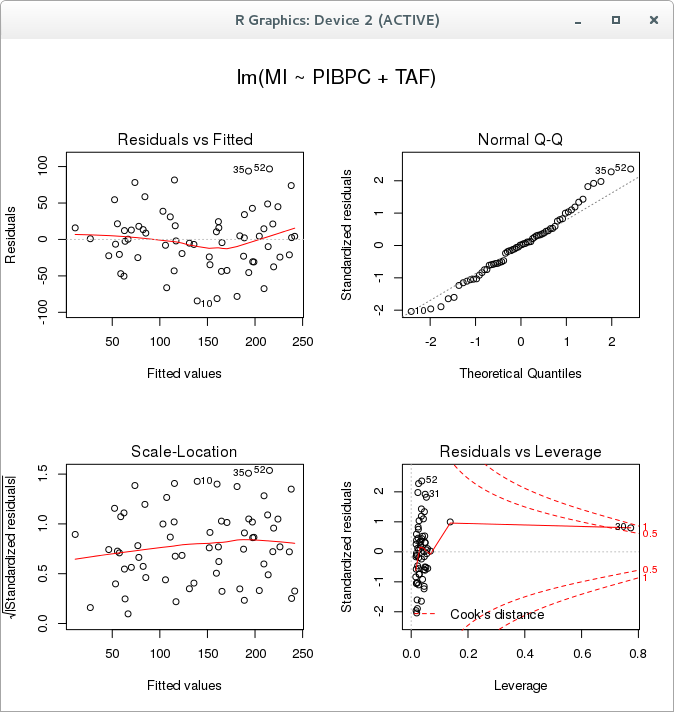
\includegraphics[width=0.9\linewidth]{analisisGraficoModelo3}\\
\caption[Titulo en el índice de figuras (opcional)]{Título en el 
documento. Las imágenes pueden ser raster (de preferencia jpg, png 
con buena resolución para imprimir) o vectorial (convertir a pdf, en 
este caso la resolución no afecta) Fuente: imagen tomada de~\cite{liu}.}
\end{figure}


\begin{lem}\label{lmcp11}Sean $z,w \in \C$, $1 < p \leq 2$ y $1/p +
1/q = 1$. Entonces tenemos \[\abs{z+w}^q + \abs{z-w}^q \leq 2 (|z|^p
+ |w|^p)^{\frac{1}{p-1}}.\]
\end{lem}

\begin{proof} Consultar~\cite[p. 227]{Hewit}. \end{proof}

\begin{defn}\label{dfcp5}Sea $f:X\To \RR$ una aplicación. Se definen
las aplicaciones $f^+\!\df\max\{f,0\}$, $f^-\!\df-\min\{f,0\}$, a
$f^+$ y $f^-$ se les llama la \textbf{parte positiva y negativa} de
$f$, respectivamente.
\end{defn}


\begin{prp}\label{prcp2}Para cualquier aplicación $f:X\To \R$
denotaremos su valor absoluto con $\abs f$, entonces tenemos
\[\abs f=f^++f^-,\quad f=f^+-f^-.\]
\end{prp}

% --------------->  

\section{Tablas y Gráficas}

Las tablas y gráficas deben tener un título \verb|\caption{text}| que la identifique, debe especificar la \textbf{fuente}, y una etiqueta \verb|\label{text}| para hacer referencias cruzadas dentro del documento.

%% TABLAS LARGAS LLEVAN TODAS LAS DIVISIONES DE LOS BLOQUES
\subsection{Tablas}

\begin{longtable}{|l|l|l|l|l|}
\caption[]{Diccionario de datos, tabla \textit{marn} (continuación)} \\ \hline

\multicolumn{1}{|c|}{\textbf{Name}} & \multicolumn{1}{c|}{\textbf{Data type}} & \multicolumn{1}{c|}{\textbf{Not Null?}} & \multicolumn{1}{c|}{\textbf{Primary key?}} & \multicolumn{1}{c|}{\textbf{Default}} \\ \hline \endhead
	\caption[Diccionario de datos, tabla \textit{marn}]{Diccionario de datos, tabla \textit{marn}. Fuente: obtenida de pgAdminIII}\label{data:marn} \\ \hline

	\multicolumn{1}{|c|}{\textbf{Name}} & \multicolumn{1}{c|}{\textbf{Data type}} & \multicolumn{1}{c|}{\textbf{Not Null?}} & \multicolumn{1}{c|}{\textbf{Primary key?}} & \multicolumn{1}{c|}{\textbf{Default}} \\ \hline \endfirsthead 

	id & \textit{integer} & \textit{Yes} & \textit{Yes} & \textit{nextval('marn\_id\_seq'} \\ %\hline

	 &  &  &  & \textit{::regclass)}\footnote{Note que la tabla es mas ancha que lo preestablecido. Procure diseñar elementos acordes con el espacio preestablecido.} \\ \hline

	\multicolumn{ 5}{|l|}{Clave primaria que  obtendrá su valor de forma secuencial al ingresar un nuevo registro} \\ \hline
		lista\_tax & \textit{text} & \textit{No} & \textit{No} & \textit{} \\ \hline

	\multicolumn{ 5}{|l|}{Clasificación del proyecto en base al Listado Taxativo del MARN} \\ \hline
		no\_marn & \textit{text} & \textit{No} & \textit{No} & \textit{} \\ \hline

	\multicolumn{ 5}{|l|}{Numero de expediente asignado por el MARN} \\ \hline
		date0 & \textit{date} & \textit{No} & \textit{No} & \textit{} \\ \hline

	\multicolumn{ 5}{|l|}{Día del ingreso del expediente del proyecto (instrumento ambiental) en el MARN} \\ \hline
		notas & \textit{text} & \textit{No} & \textit{No} & \textit{} \\ \hline

	\multicolumn{ 5}{|l|}{Observaciones} \\ \hline
		no\_res\_ap & \textit{text} & \textit{No} & \textit{No} & \textit{} \\ \hline

	\multicolumn{ 5}{|l|}{Numero de resolución aprobatoria del proyecto por el MARN%
	\footnote{Note que en esta línea la tabla se corta y continua en la siguiente página. 
	Utilizar paquete \textsf{longtable} y ambiente \textit{longtable}.}} \\ \hline
		date\_res\_ap & \textit{date} & \textit{No} & \textit{No} & \textit{} \\ \hline

	\multicolumn{ 5}{|l|}{Día de emisión de la resolución aprobatoria por el MARN} \\ \hline
		date0\_fianza & \textit{date} & \textit{No} & \textit{No} & \textit{} \\ \hline

	\multicolumn{ 5}{|l|}{Día de emisión de fianza del proyecto.} \\ \hline
		no\_res\_fianza & \textit{text} & \textit{No} & \textit{No} & \textit{} \\ \hline

	\multicolumn{ 5}{|l|}{Numero de la resolución de aceptación de fianza por el MARN} \\ \hline
		date1\_fianza & \textit{date} & \textit{No} & \textit{No} & \textit{} \\ \hline

	\multicolumn{ 5}{|l|}{Fecha de inicio de fianza} \\ \hline
		date2\_fianza & \textit{date} & \textit{No} & \textit{No} & \textit{} \\ \hline

	\multicolumn{ 5}{|l|}{Fecha de finalización de fianza (renovación)} \\ \hline
		lic\_ambiental & \textit{text} & \textit{No} & \textit{No} & \textit{} \\ \hline

	\multicolumn{ 5}{|l|}{Numero de licencia ambiental} \\ \hline
		date\_lic\_ambiental & \textit{date} & \textit{No} & \textit{No} & \textit{} \\ \hline

	\multicolumn{ 5}{|l|}{Fecha de finalización de ultima licencia ambiental} \\ \hline
		proyecto\_id & \textit{integer} & \textit{Yes} & \textit{No} & \textit{} \\ \hline

	\multicolumn{ 5}{|l|}{Enlace con la tabla proyecto\_id} \\ \hline
\end{longtable}




\par}               % termina interlineado 1 1/2

\end{document}

%%% Local Variables:
%%% TeX-master: t 
%%% End: